\newpage
\section{Конструкторская часть}

Рассмотрим алгоритм полного перебора и муравьиный алгоритм.

\subsection{Функциональная модель}

На рисунке \ref{img:idef0} представлена функциональная модель IDEF0
первого уровня, а на рисунке \ref{img:idef0_2} IDEF0 второго уровня.

\begin{figure}[H]
    \centering
    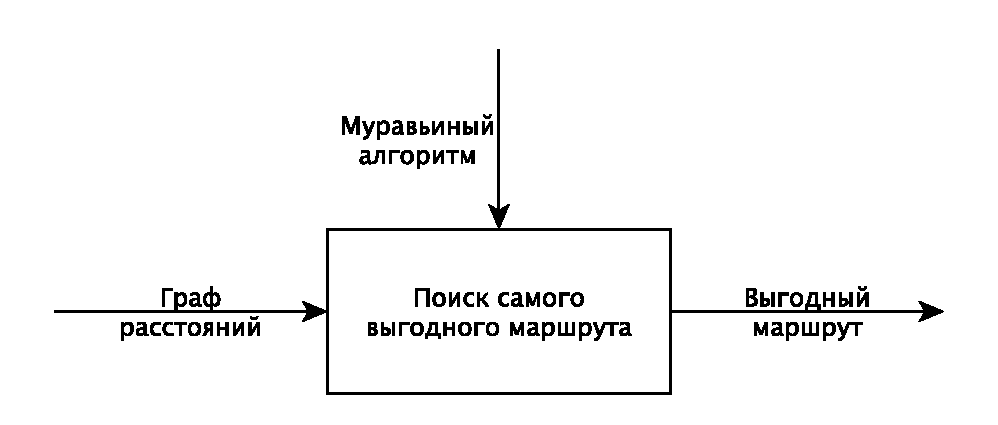
\includegraphics[scale=0.9]{idef0}
    \caption{IDEF0 первого уговня}
    \label{img:idef0}
\end{figure}

\begin{figure}[H]
    \centering
    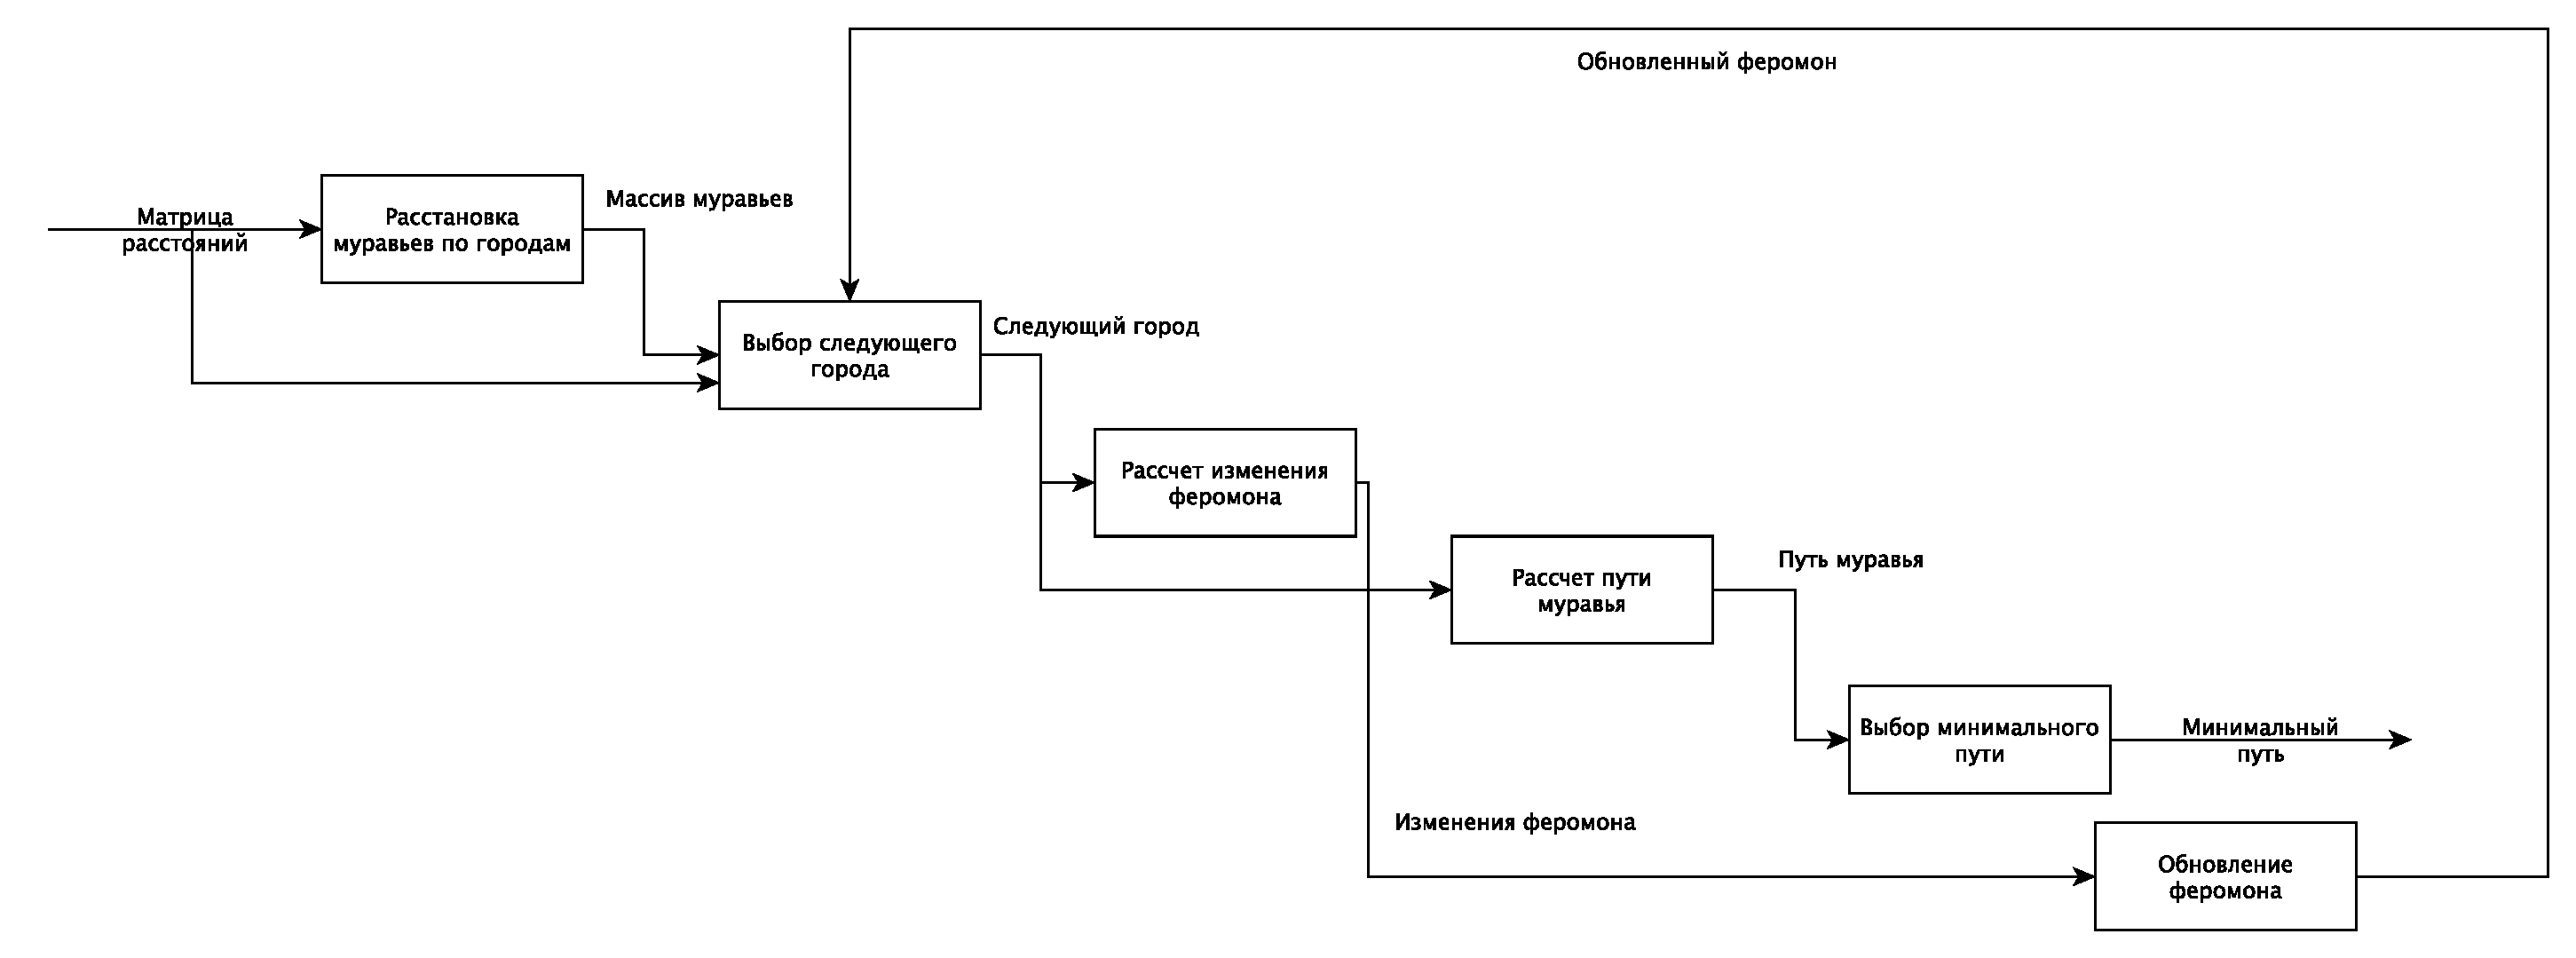
\includegraphics[scale=0.3]{idef0_lvl2}
    \caption{IDEF0 второго уговня}
    \label{img:idef0_2}
\end{figure}

\subsection{Схемы алгоритмов}

На рисунке \ref{img:ant} представлена схема муравьиного алгоритма.

\begin{figure}[H]
    \centering
    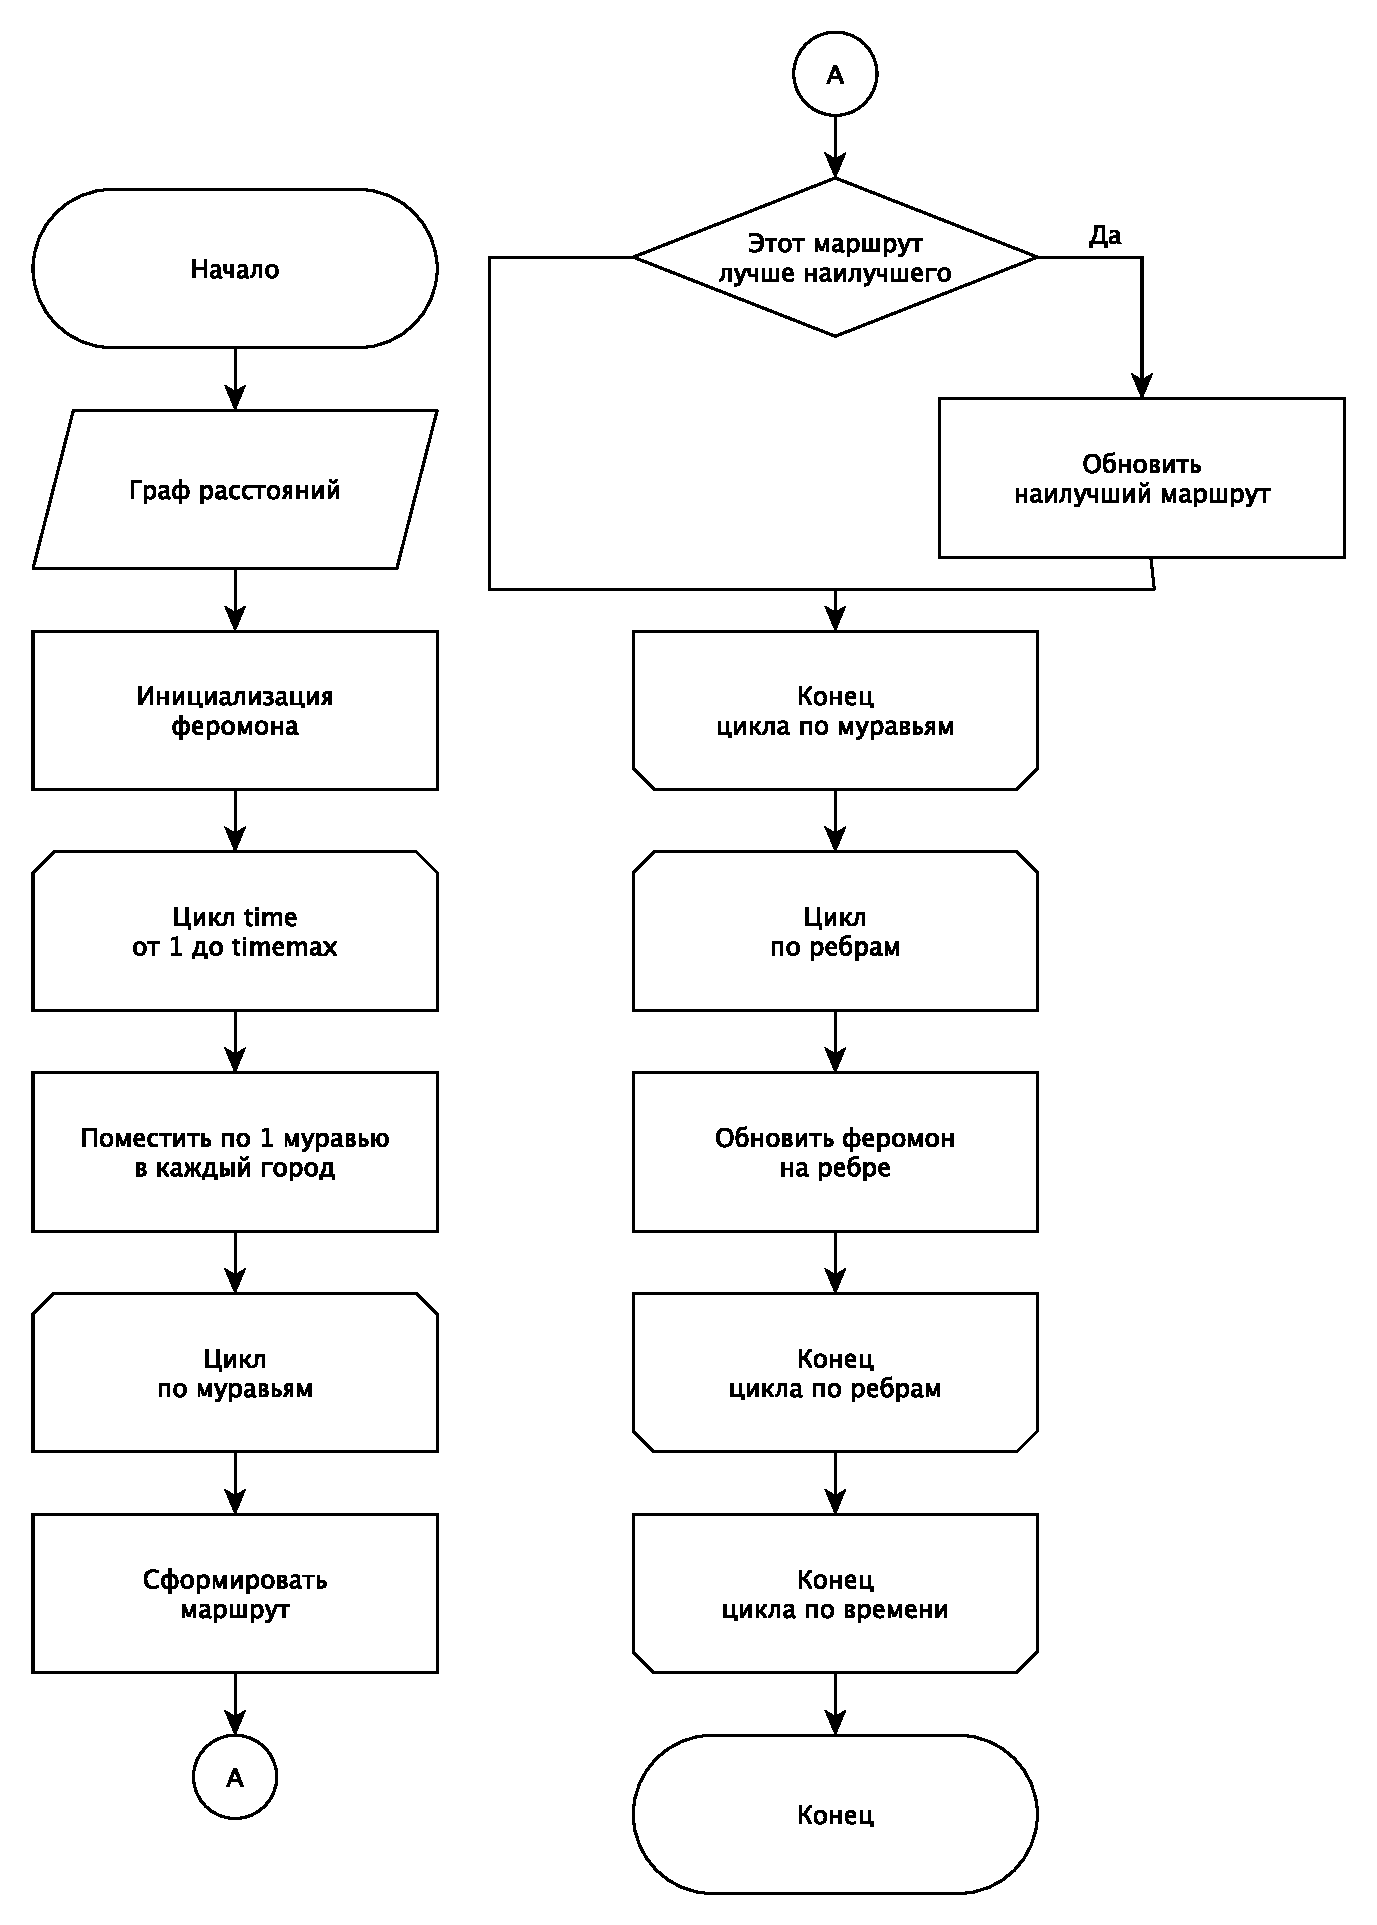
\includegraphics[scale=0.7]{ant}
    \caption{Схема муравьиного алгоритма}
    \label{img:ant}
\end{figure}

\subsection{Выводы}

Необходимо разработать данный алгоритм, провести тестирование и исследование, сравнив с
алгоритмом полного перебора.
